\documentclass{article}

% So that TeX doesn't complain about small
% underfull or overfull boxes
\hfuzz1pc
% Make the overfull marker bigger
\overfullrule=2cm

% Font setup.
\usepackage{unicode-math}
\setmainfont{STIX Two Text}
\setsansfont[Scale=MatchLowercase]{Source Sans 3}
\setmonofont[Scale=MatchLowercase]{Ubuntu Mono}
\setmathfont[Scale=.93]{STIX Two Math}
\linespread{1.05}
% Don't put extra space after periods
\frenchspacing
\KOMAoptions{
    paper = letter,
    BCOR = 0mm,
    twoside = false,
    fontsize = {8},
    DIV = calc,
}

% Make bibliography more compact, no indents.
\KOMAoption{toc}{flat}

% Language support, usually changes between english
% and spanish.
\usepackage[spanish,es-noindentfirst]{babel}
%\usepackage[english]{babel}
\usepackage{csquotes}

% Bibliography
\usepackage[
    backend=biber,
    style=numeric-comp,
    backref=true,
    backrefstyle=two,
    abbreviate=true
]{biblatex}
\addbibresource{~/git/Misc-LaTeX-files/bib/general.bib}
\addbibresource{~/git/Misc-LaTeX-files/bib/math-books.bib}

% Graphics, mainly to insert images or
% single page PDFs.
\usepackage{graphicx}
\usepackage[dvipsnames]{xcolor}
% Handy command to typeset URLs
\usepackage{hyperref}
\hypersetup{
    colorlinks=true,
    linkcolor=Mahogany,
    filecolor=Mahogany,
    urlcolor=Black,
    citecolor=Mahogany,
}
\usepackage{url}
%\urlstyle{same}
\usepackage{metalogo}

%\usepackage{minted}

% Font style and size for title
\setkomafont{title}{\itshape}
% Font style for the subject
\setkomafont{subject}{\normalfont}
% Font style for subtitle
\setkomafont{subtitle}{\normalfont\itshape}
\setkomafont{author}{\large}
\setkomafont{date}{\normalsize}
\setkomafont{section}{\fontseries{m}\Large}
\setkomafont{subsection}{\fontseries{m}\large}
\setkomafont{subsubsection}{\fontseries{m}\normalsize}

% Footnotes
\deffootnote{2.0em}{1.5em}{\thefootnotemark.\ }
\setkomafont{footnote}{\sffamily}

\newcounter{exer}
\newcommand{\exercise}{%
    \stepcounter{exer}%
    \begin{center}%
        \addfontfeatures{LetterSpace=7}\large\Roman{exer}%
    \end{center}%
}
\newcommand{\solution}{
    \begin{center}
        Solución
    \end{center}
}

% CUSTOM MACROS
% math macros
\renewcommand{\Rn}{\mathbb{R}^{\mathrm{n}}}
\newcommand{\Rm}{\mathbb{R}^{\mathrm{m}}}
\newcommand{\R}{\mathbb{R}}
\newcommand{\N}{\mathbb{N}}
\newcommand{\devpart}[2]{\frac{\partial  #1}{\partial #2}}
\renewcommand{\vec}[1]{\mathbf{#1}}
\newcommand{\norm}[1]{\left\lvert #1 \right\rvert}
\newcommand{\iprod}[2]{\left\langle #1 , #2 \right\rangle}
\newcommand{\devp}[2]{\frac{\partial #1}{\partial #2}}
\DeclareMathOperator{\img}{img}
\DeclareMathOperator{\gen}{span}


\errorstopmode

\newcommand{\comment}[1]{\text{\small #1}}

\begin{document}
%
\title{Primer Parcial}
% \subtitle{Septiembre-Diciembre 2021}
% \subject{Análisis IV}
% \titlehead{Universidad Simón Bolívar\hfill Caracas, Venezuela}
\author{Jhonny Lanzuisi}
\date{\today}
\maketitle

\exercise
Sean $z, w \in \Cplx$. Demuestre que
\[
    |z + w| = |z| + |w|
\]
si y sólo si $z \overline{w}$ es un número real no negativo.

\solution
Sean $z = a_1 + ia_2$ y $w = b_1 + ib_2$, entonces:
\allowdisplaybreaks
\begin{gather*}
    |z + w| = |z| + |w| \\
    \iff\comment{(Definición del valor absoluto)} \\
    \sqrt{(a_1 + b_1)^2 + (a_2 + b_2)^2}
        = \sqrt{a_1^2 + a_2^2} + \sqrt{b_1^2 + b_2^2} \\
    \iff\comment{(Elevando al cuadrado)}\\
    (a_1 + b_1)^2 + (a_2 + b_2)^2
        = a_1^2 + a_2^2 + b_1^2 + b_2^2
            + 2 \sqrt{a_1^2 + a_2^2} \sqrt{b_1^2 + b_2^2}\\
    \iff\comment{(Expandiendo lado izquierdo)}\\
    a_1^2 + 2a_1b_1 + b_1^2 + a_2^2 + 2a_2b_2 + b_2^2
            = a_1^2 + a_2^2 + b_1^2 + b_2^2
                + 2 \sqrt{a_1^2 + a_2^2} \sqrt{b_1^2 + b_2^2}\\
    \iff\comment{(Simplificando)}\\
    a_1b_1 + a_2b_2 = \sqrt{a_1^2 + a_2^2} \sqrt{b_1^2 + b_2^2}\\
    \iff\comment{(Elevando al cuadrado)}\\
    (a_1b_1 + a_2b_2)^2 = (a_1^2 + a_2^2) (b_1^2 + b_2^2)\\
    \iff\comment{(Expandiendo multiplicaciones)}\\
    a_1^2b_1^2 + 2a_1b_1a_2b_2 + a_2^2b_2^2
        = a_1^2b_1^2 + a_1^2b_2^2 + a_2^2b_1^2 + a_2^2b_2^2\\
    \iff\comment{(Simplificando)}\\
    2a_1b_1a_2b_2 = a_1^2b_2^2 + a_2^2b_1^2\\
    \iff\\
    0 = (a_1b_2)^2 + 2(a_1b_2)(a_2b_1) + (a_2b_1)^2\\
    \iff\\
    0 = (a_1b_2 - a_2b_1)^2\\
    \iff\\
    0 = a_1b_2 - a_2b_1
\end{gather*}

Pero el lado derecho de la última igualdad es la parte compleja
de $z\overline{w}$. Tomando en cuenta esto y que todas las implicaciones son dobles,
hemos demostrado lo que buscábamos.

\exercise
Considere $S$ como el conjunto que consiste en retirar del
plano complejo la circunferencia de centro en el origen y radio $\sqrt5$.
Considerando $S \cup \partial S$, es $S$ un conjunto conexo?

\solution
Sea $C = \{ z\in\Cplx\colon |z| \leq \sqrt{5} \}$ la circunferencia del enunciado.
Entonces $S = \Cplx\setminus C$, es decir, $S = \{ z\in\Cplx\colon |z| > \sqrt{5} \}$.
La frontera de $S$ es el conjunto en el cual cualquier bola abierta centrada en cualquiera de
sus puntos, contiene elementos dentro y fuera de $S$.
Se sigue que $\partial S = \{z\in\Cplx\colon |z| = \sqrt{5}\}$.
Obtenemos entonces $S\cup\partial S = \{ z\in\Cplx\colon |z| \geq \sqrt{5} \}$.

Queremos ahora demostrar que, dados dos puntos $s_1,s_2\in S\cup\partial S$, existe un conjunto
de segmentos contiguos (polígono) que los unen.

Consideremos la circunferencia $C_1$ de centro en el orígen y radio $|s_1|$ y también la
circunferencia $C_2$ de centro en el orígen y radio $|s_2|$.
Distinguimos ahora dos casos:
\begin{enumerate}
    \item Existe una recta $\ell$ que pasa por el orígen y contiene a los puntos $s_1$ y $s_2$, ó,
    \item No existe tal recta $\ell$, y por lo tanto los puntos $s_1,s_2$ no son
        diametralmente opuestos con respecto al orígen.
\end{enumerate}

Podemos construir un polígono que uno a los puntos $s_1,s_2$ dependiendo del caso que nos encontremos.

\begin{description}
    \item[Caso 2] (Figura 1) Tomemos la recta $L_1$ tangente a $C_1$ en $s_1$ y la recta $L_2$ tangente a $C_2$ en $s_2$.
        Estas rectas, no paralelas, se intersectan en un punto $w$. El polígono $[s_1,w]\cup[w,s_2]$ esta totalmente
        contenido en $S\cup\partial S$. De no estar totalmente contenido, algún punto de dicho polígono estaría en la región
        $C^\ast = \{z\in\Cplx\colon |z| < \sqrt{5}\}$, pero esto es imposible puesto que $C^\ast\subset C_1$ y $C^\ast\subset C_2$
        por lo que los segmentos $[s_1,w],[w,s_2]$ nunca intersectan a $C^\ast$ pues dichos segmentos tocan a $C_1,C_2$
        en $s_1,s_2$, respectivamente, y no en ningún otro punto. Al $s_1,s_2$ no ser puntos de $C^\ast$, se tiene que el
        polígono propuesto esta completamente contenido en $S\cup\partial S$.
    \item[Caso 1] (Figura 2) En este caso $L_1$ y $L_2$ son paralelas. Tomemos una perpendicular $P$ a $L_1$ tal que $|s_1-w_1| > \sqrt{5}$,
        donde $w_1$ es la intersección de $P$ con $L_1$. Como $L_1$ y $L_2$ son paralelas, $P$ intersecta a $L_2$ en un punto
        $w_2$. El polígono $[s_1,w_1]\cup[w_1,w_2]\cup[w_2,s_2]$ esta totalmente contenido en $S\cup\partial S$. Los segmentos
        $[s_1,w_1],[w_2,s_2]$ no contienen ningún punto de $C^\ast$ por las mismas razones que el caso anterior. El segmento
        $[w_1,w_2]$, al ser $|s_1-w| > \sqrt{5}$, es tal que $|z| > \sqrt{5}\;\forall z\in[w_1,w_2]$, y entonces dicho segmento
        no posee nigún punto de $C^\ast$.
\end{description}

Hemos demostrado que, en cualquier caso, existe un polígono que une a dos puntos cualesquiera de $S\cup\partial S$
por lo que este conjunto es conexo.

\begin{figure}
    \begin{center}
        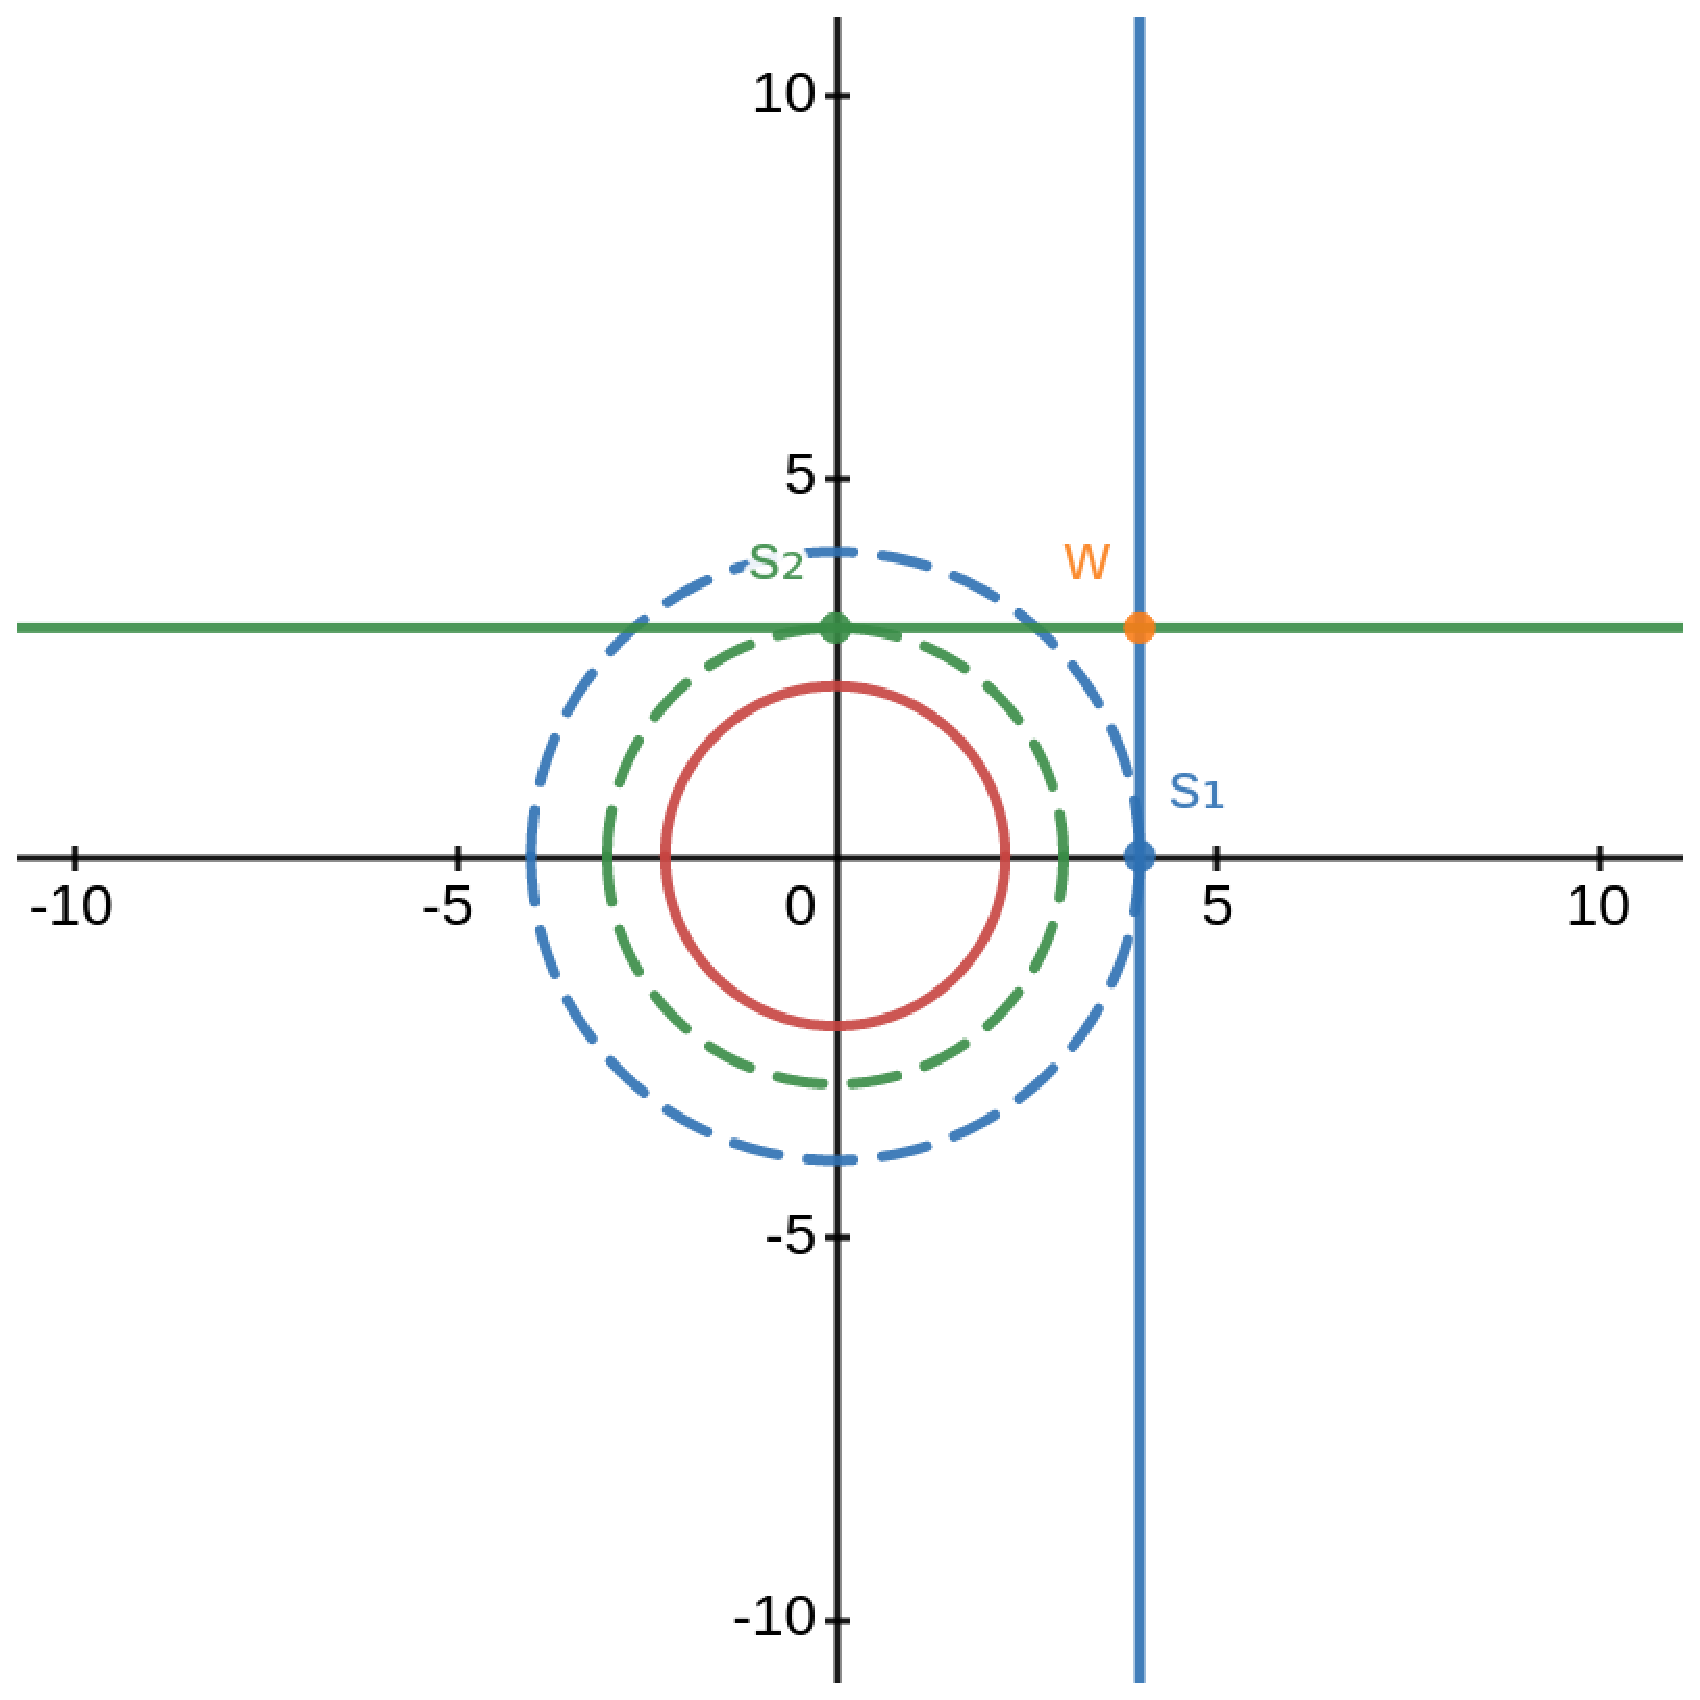
\includegraphics[width=.65\textwidth]{caso2}
    \end{center}
    \caption{Segundo caso.}
\end{figure}
%
\begin{figure}
    \begin{center}
        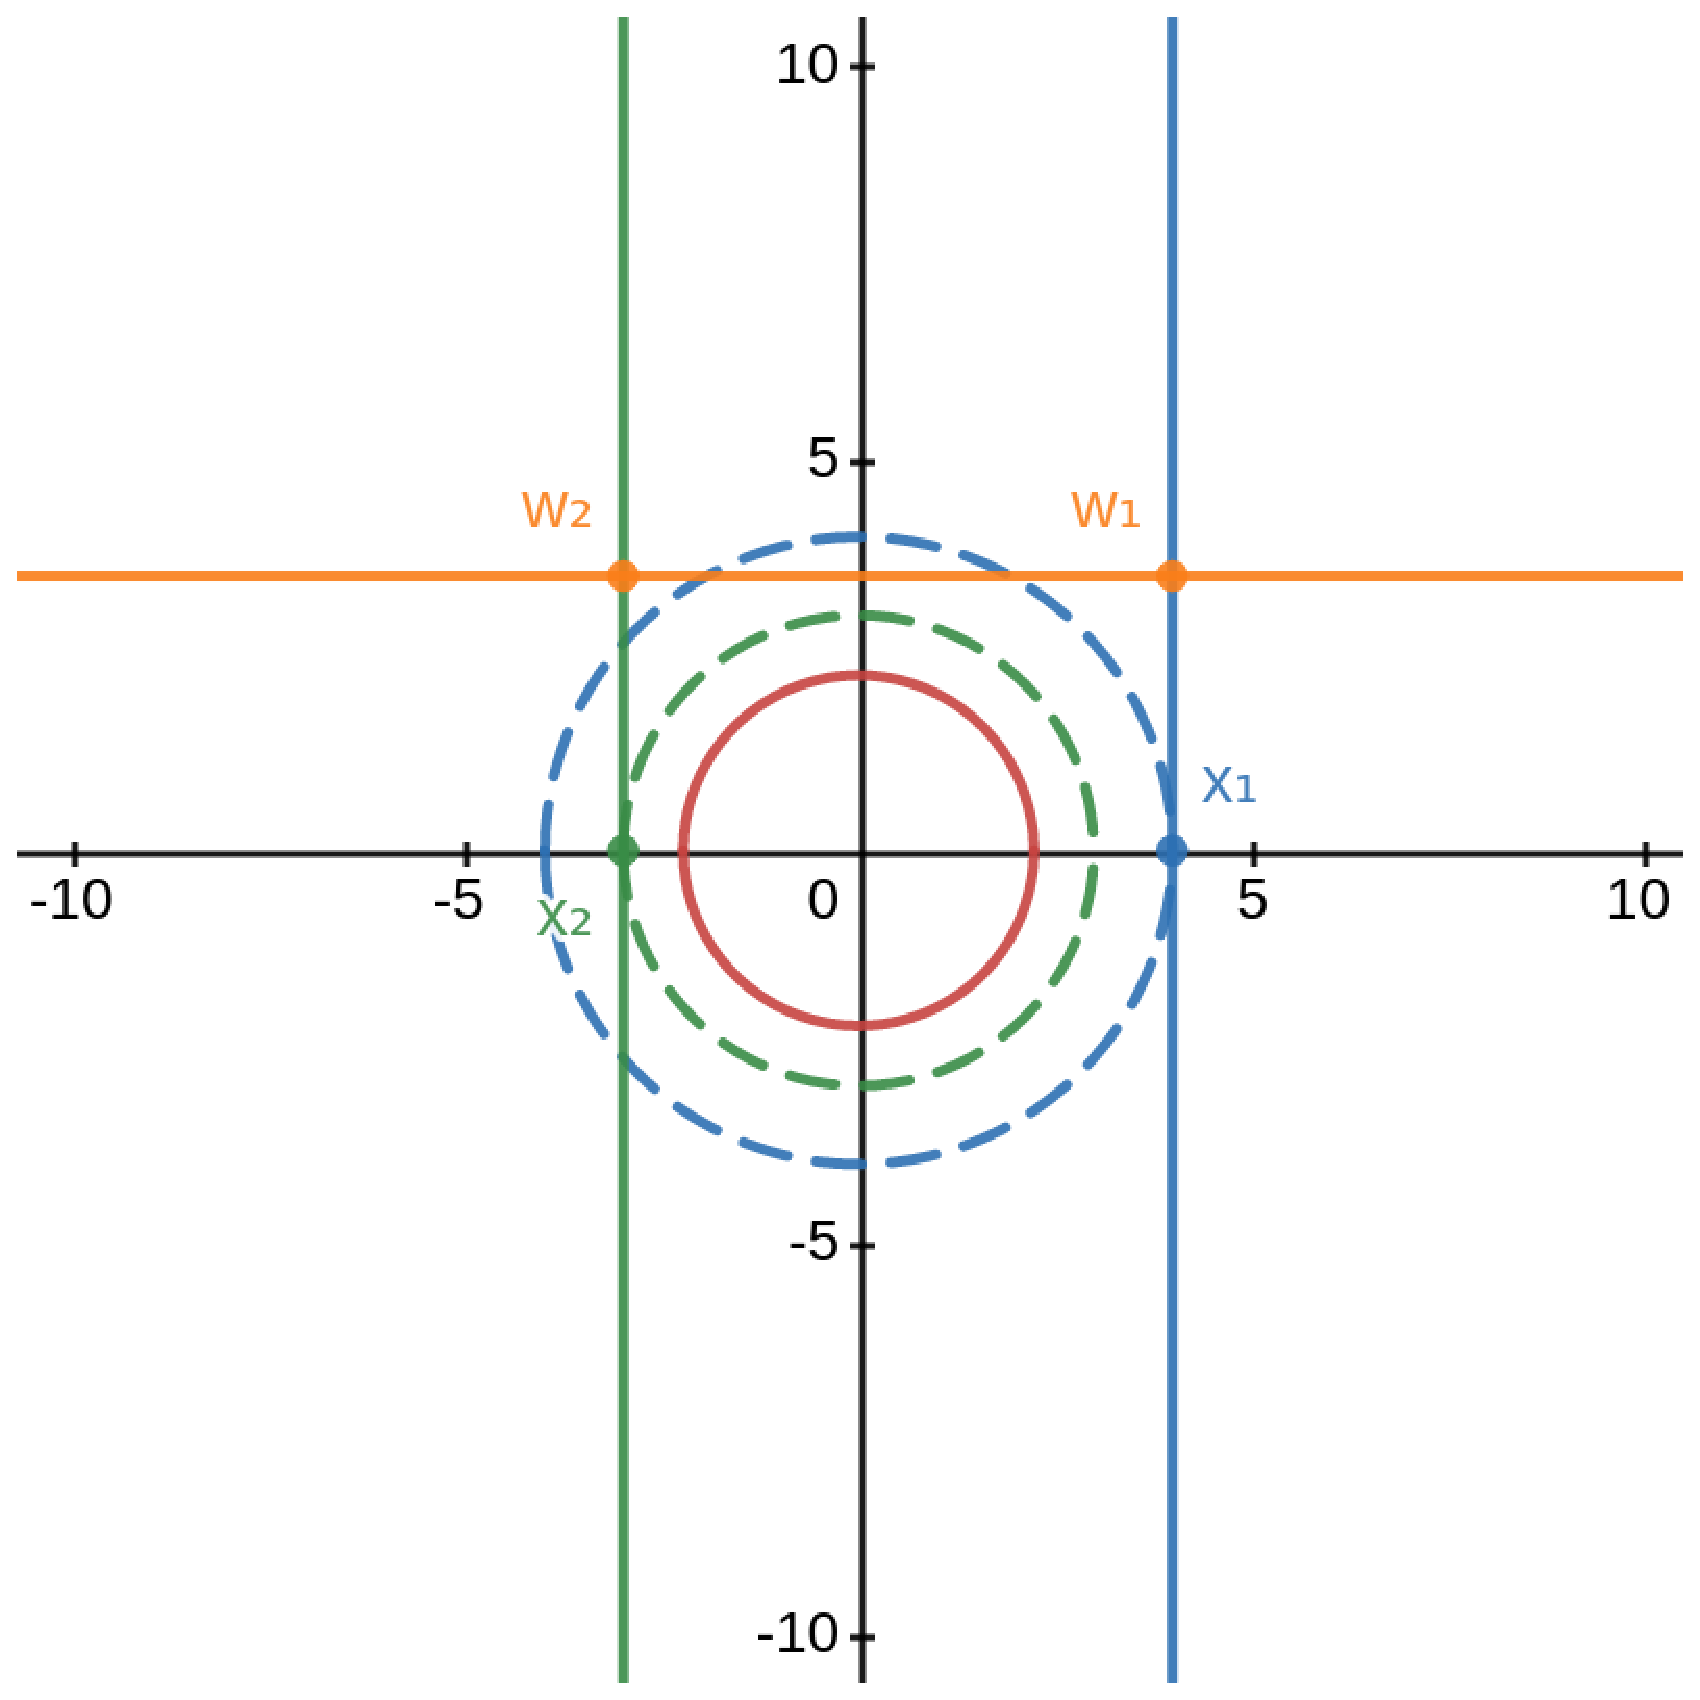
\includegraphics[width=.65\textwidth]{caso1}
    \end{center}
    \caption{Primer caso.}
\end{figure}

%\printbibliography
\newpage
\section*{Colophon \& Copyright}
This document was typeset using \TeX%
\footnote{%
    \TeX\ is
    a typesetting software, free and open source,
    developed by Donald Knuth. \LaTeX\ is a macro
    set for \TeX\ developed by Leslie Lamport. \LuaTeX\ is
    a reworking of \TeX\ adding native support for the Lua
    programming language and unicode, among other things.
    All of them are available in all major
    operating systems.
}
and the \LaTeXe\ macros in a GNU/Linux system.
The editor used for editing the text was Visual Studio Code.%
The main typeface used is the STIX Two family%
\footnote{%
    The STIX typefaces were design for technical typesetting,
    and they include both text and math fonts.
}
for text and math,
the sans-serif typeface is Source Sans by Adobe%
\footnote{%
    This is a free and open source typeface comissioned by Adobe.
}.

\medskip
%
\begin{quote}
\sffamily\small
     E-mail: \url{jalb97@gmail.com}. \\
    Copyright (C) 2021 Jhonny Lanzuisi. \\
    This work is licensed under the Creative Commons Attri\-bu\-tion-Sha\-re\-Alike
    International (CC BY-SA 4.0)  License. To view a copy of the license,
    visit \url{https://creativecommons.org/licenses/by-sa/4.0/}.
\end{quote}

\end{document}
